\documentclass[preprint,12pt]{elsarticle}

\usepackage{graphicx}
\usepackage{amsmath,amssymb}
\usepackage{booktabs}
\usepackage{siunitx}
\usepackage{hyperref}
% natbib loaded by elsarticle

\graphicspath{{../results/}{../benchmark/images/}}

\journal{Draft — Target Journal TBD}

\begin{document}

\begin{frontmatter}

\title{Can Vision-Language Models Evaluate CFD? A Benchmark for Physical Plausibility Assessment of Flow Field Visualizations}

\author[1]{Author One\corref{cor1}}
\ead{author@institution.edu}
\author[1]{Author Two}

\cortext[cor1]{Corresponding author}
\address[1]{Institution, Department, City, Country}

\begin{abstract}
Validating computational fluid dynamics (CFD) simulation results remains a manual bottleneck in automated pipelines, requiring expert visual inspection of flow field images. We introduce CFD-VisQA, the first benchmark for evaluating vision-language model (VLM) capabilities in assessing physical plausibility of CFD visualizations. The benchmark comprises 10 canonical thermal-fluid scenarios with 60 OpenFOAM cases, 258 flow field images, and 279 physics-grounded questions at 5 difficulty levels. Each scenario includes correct solutions and systematically generated errors spanning 6 types at varying severity levels. Using a blind, setup-conditioned protocol with anonymized case identifiers, we evaluate Claude Opus 4.6 (75 items, 3 independent trials), Gemini 3.1 (30 items, 3 trials), and a domain expert (80 items). Claude Opus achieves 99.6\% accuracy across 225 judgments (majority vote: 100\%), compared to 73.8\% for the domain expert and 87.5\% mean accuracy for Gemini 3.1. The expert primarily misses ``subtle'' errors that produce plausible-looking flows (boundary condition swaps: 20\% recall, wrong viscosity: 29\% recall), while Claude detects these through systematic cross-referencing of setup text against visual features. We document a contamination paradox where providing case-name metadata decreases VLM accuracy (87\% vs.\ 100\% blind), and show that per-item consistency across 3 trials reaches 98.7\% for Claude. These findings suggest that frontier VLMs show promise as automated CFD validators with error detection patterns complementary to human experts, though evaluation scope and model coverage require further expansion. The benchmark dataset and evaluation pipeline are publicly available.
\end{abstract}

\begin{keyword}
vision-language model \sep computational fluid dynamics \sep benchmark \sep flow visualization \sep physical plausibility \sep automated validation
\end{keyword}

\end{frontmatter}

\section{Introduction}

Computational fluid dynamics (CFD) is increasingly integrated into automated design and analysis pipelines, from building ventilation assessment to industrial heat exchanger optimization. Recent advances in vision-language models (VLMs) have enabled new paradigms such as image-to-CFD frameworks, where a VLM extracts geometric information from architectural images to automatically generate CFD simulation domains \cite{joo2026}. As these automated pipelines proliferate, a critical bottleneck emerges: \textit{who validates the results?}

In traditional CFD workflows, an experienced engineer inspects velocity contours, temperature fields, and streamline plots to confirm that the solution is physically reasonable, checking for proper boundary layer development, expected recirculation patterns, and absence of numerical artifacts. This visual inspection requires domain expertise accumulated over years and cannot scale with the throughput of automated pipelines. If a VLM could perform this validation step---assessing whether a CFD flow field visualization is physically plausible---the automation loop would close entirely.

Yet it remains unknown whether current VLMs possess the physical reasoning capability to evaluate CFD output images. Existing VLM benchmarks test scientific knowledge through multiple-choice questions on textbook diagrams \cite{yue2024mmmu}, chart comprehension \cite{pandey2025}, or everyday physics understanding \cite{chow2025physbench}, but none evaluate the ability to assess simulation output images against known physical laws. The closest work evaluates VLMs on meteorological heatmaps \cite{chen2024climateIQA} or tests generative AI on fluid mechanics prompts \cite{kashefi2024}, but neither addresses the specific task of CFD result validation.

This paper introduces \textbf{CFD-VisQA}, the first benchmark designed to evaluate VLM capabilities in assessing physical plausibility of CFD flow field visualizations. The benchmark comprises 10 canonical thermal-fluid scenarios (natural convection, forced convection, mixed convection), each with correct solutions and systematically generated erroneous solutions spanning 6 error types. We evaluate two frontier VLMs (Claude Opus 4.6 and Gemini 3.1) against a domain expert using a blind, multi-trial protocol on 75--80 evaluation items, revealing distinct error detection patterns across evaluator types.

Our contributions are:
\begin{enumerate}
\item \textbf{CFD-VisQA benchmark dataset}: 60 OpenFOAM CFD cases across 10 thermal-fluid scenarios, producing 258 flow field images with 279 physics-grounded questions and expert annotations. The dataset includes both correct solutions and 6 types of intentionally generated errors at varying severity levels.
\item \textbf{Setup-conditioned evaluation protocol}: We demonstrate that providing problem setup text alongside the image (boundary conditions, Reynolds number, solver type) dramatically improves VLM performance compared to image-only evaluation, and introduce a blind evaluation protocol that prevents bias from case-name leakage.
\item \textbf{Comparative analysis revealing differential blind spots}: Claude Opus achieves 98.7\% accuracy on 75 items (99.6\% across 3 trials, majority vote 100\%), the domain expert 73.8\% on 80 items, and Gemini 3.1 87.5\% mean on 30 items. Each evaluator misses different error types, suggesting complementary strengths.
\item \textbf{Multi-trial consistency and contamination paradox}: Three independent blind trials show 98.7\% per-item consistency for Claude. Providing case-name metadata decreases VLM accuracy (87\% contaminated vs.\ 100\% blind), demonstrating that evaluation protocol design materially affects results.
\end{enumerate}

\section{Related Work}

\subsection{VLM Benchmarks for Scientific Visuals}

Several benchmarks evaluate VLM performance on scientific and technical imagery, though none address CFD specifically. MMMU \cite{yue2024mmmu} tests college-level reasoning across 30 disciplines with 11,500 questions, including engineering diagrams, but contains no flow field images. SciFIBench \cite{roberts2024} evaluates 28 large multimodal models on 2,000 scientific figure interpretation tasks from arXiv papers, finding that VLM capabilities in scientific figure understanding are ``not well characterised.'' PhysBench \cite{chow2025physbench} tests 75 VLMs on physical world understanding across 10,002 entries, finding that the best model (GPT-4o) achieves only 49.5\% vs.\ 95.9\% human accuracy; however, its ``fluid dynamics'' category covers everyday scenarios (water pouring) rather than simulation outputs.

Most relevant to our work is ClimateIQA \cite{chen2024climateIQA}, which constructs 26,280 meteorological heatmap images with 762,120 instruction samples for VLM evaluation. Like CFD contour plots, meteorological heatmaps require colormap interpretation and spatial pattern recognition. We extend this line of work from meteorological to engineering simulation imagery, with the additional challenge of physics-grounded plausibility assessment.

\subsection{AI for CFD Result Assessment}

The intersection of AI and CFD has been explored primarily through surrogate modeling and simulation automation, not result validation. CFDLLMBench \cite{somasekharan2025} evaluates LLMs on CFD knowledge (92\% on conceptual MCQs) and OpenFOAM case generation (25--34\% success), but includes no visual component. The only published work directly evaluating VLMs on CFD visualizations is a 2026 study on mixed-reality indoor CFD images \cite{mdpi2026vlmcfd}, which fine-tunes Qwen2.5-VL from $<$30\% to $>$60\% accuracy on domain-specific questions. Kashefi \cite{kashefi2024} demonstrates that generative AI systems produce physically incorrect fluid mechanics imagery, motivating the need for a public CFD visualization benchmark.

\subsection{Research Gap}

No existing benchmark evaluates VLM capability to assess physical plausibility of CFD simulation output images. CFD-VisQA fills this gap with a dedicated benchmark combining physics-grounded questions, systematically generated errors, and a blind evaluation protocol.

\section{Benchmark Design}

\subsection{Design Philosophy}

The CFD-VisQA benchmark is built on three principles. First, it must measure a spectrum of visual understanding capabilities, from basic colorbar reading to physics-grounded plausibility assessment. Second, it requires both correct and intentionally erroneous flow fields. Third, all data must be reproducible: every flow field is generated from OpenFOAM simulations with published scripts. The benchmark is organized along three orthogonal axes (Fig.~\ref{fig:benchmark-overview}): flow scenarios, visualization types, and question difficulty levels.

\begin{figure}[htbp]
\centering
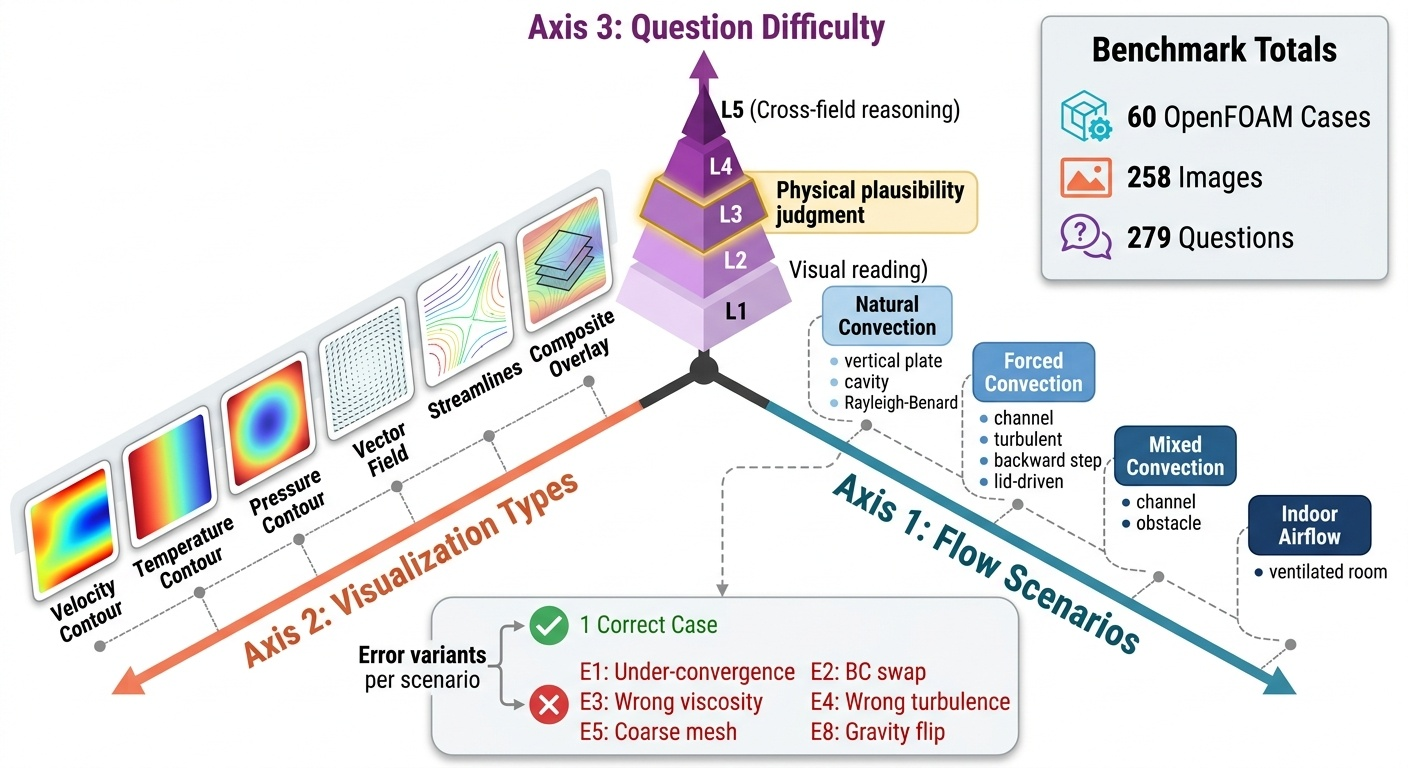
\includegraphics[width=\textwidth]{fig_benchmark_overview.png}
\caption{CFD-VisQA benchmark structure organized along three axes: 10 flow scenarios, 6 visualization types, and 5 question difficulty levels, with 6 error types applied per scenario.}
\label{fig:benchmark-overview}
\end{figure}

\subsection{Flow Scenarios}

We select ten canonical thermal-fluid scenarios spanning natural convection, forced convection, and mixed convection regimes (Table~\ref{tab:scenarios}). Reynolds numbers span $10^2$--$10^4$ and Rayleigh numbers span $10^3$--$3 \times 10^7$, covering laminar and turbulent regimes. All simulations are two-dimensional, using OpenFOAM's \texttt{simpleFoam} for isothermal flows and \texttt{buoyantBoussinesqSimpleFoam} for buoyancy-driven flows.

\begin{table}[htbp]
\centering
\caption{CFD-VisQA benchmark scenarios.}
\label{tab:scenarios}
\footnotesize
\begin{tabular}{llllr}
\toprule
ID & Scenario & Physics & Solver & Cases \\
\midrule
S1 & Heated vertical plate & Natural conv. & buoyantBoussinesq & 6 \\
S2 & Channel flow (laminar) & Forced conv. & simpleFoam & 6 \\
S3 & Channel flow (turbulent) & Forced conv. & simpleFoam + SST & 6 \\
S4 & Backward-facing step & Separation & simpleFoam & 6 \\
S5 & Lid-driven cavity & Recirculation & simpleFoam & 6 \\
S6 & Differentially heated cavity & Natural conv. & buoyantBoussinesq & 6 \\
S7 & Mixed convection channel & Mixed conv. & buoyantBoussinesq & 6 \\
S8 & Heated obstacle & Wake + thermal & buoyantBoussinesq & 6 \\
S9 & Rayleigh-B\'{e}nard & Conv.\ cells & buoyantBoussinesq & 6 \\
S10 & Ventilated room & Indoor airflow & simpleFoam + SST & 6 \\
\midrule
& \textbf{Total} & & & \textbf{60} \\
\bottomrule
\end{tabular}
\end{table}

\subsection{Error Taxonomy}

We define six error types, each produced by a controlled perturbation (Fig.~\ref{fig:error-examples}): E1 under-convergence (30 iterations), E2 boundary condition swap, E3 wrong viscosity ($10$--$100\times$), E4 wrong turbulence model (laminar at turbulent Re), E5 coarse mesh (${\sim}10\times$ reduced), and E8 gravity/direction reversal.

\begin{figure}[htbp]
\centering
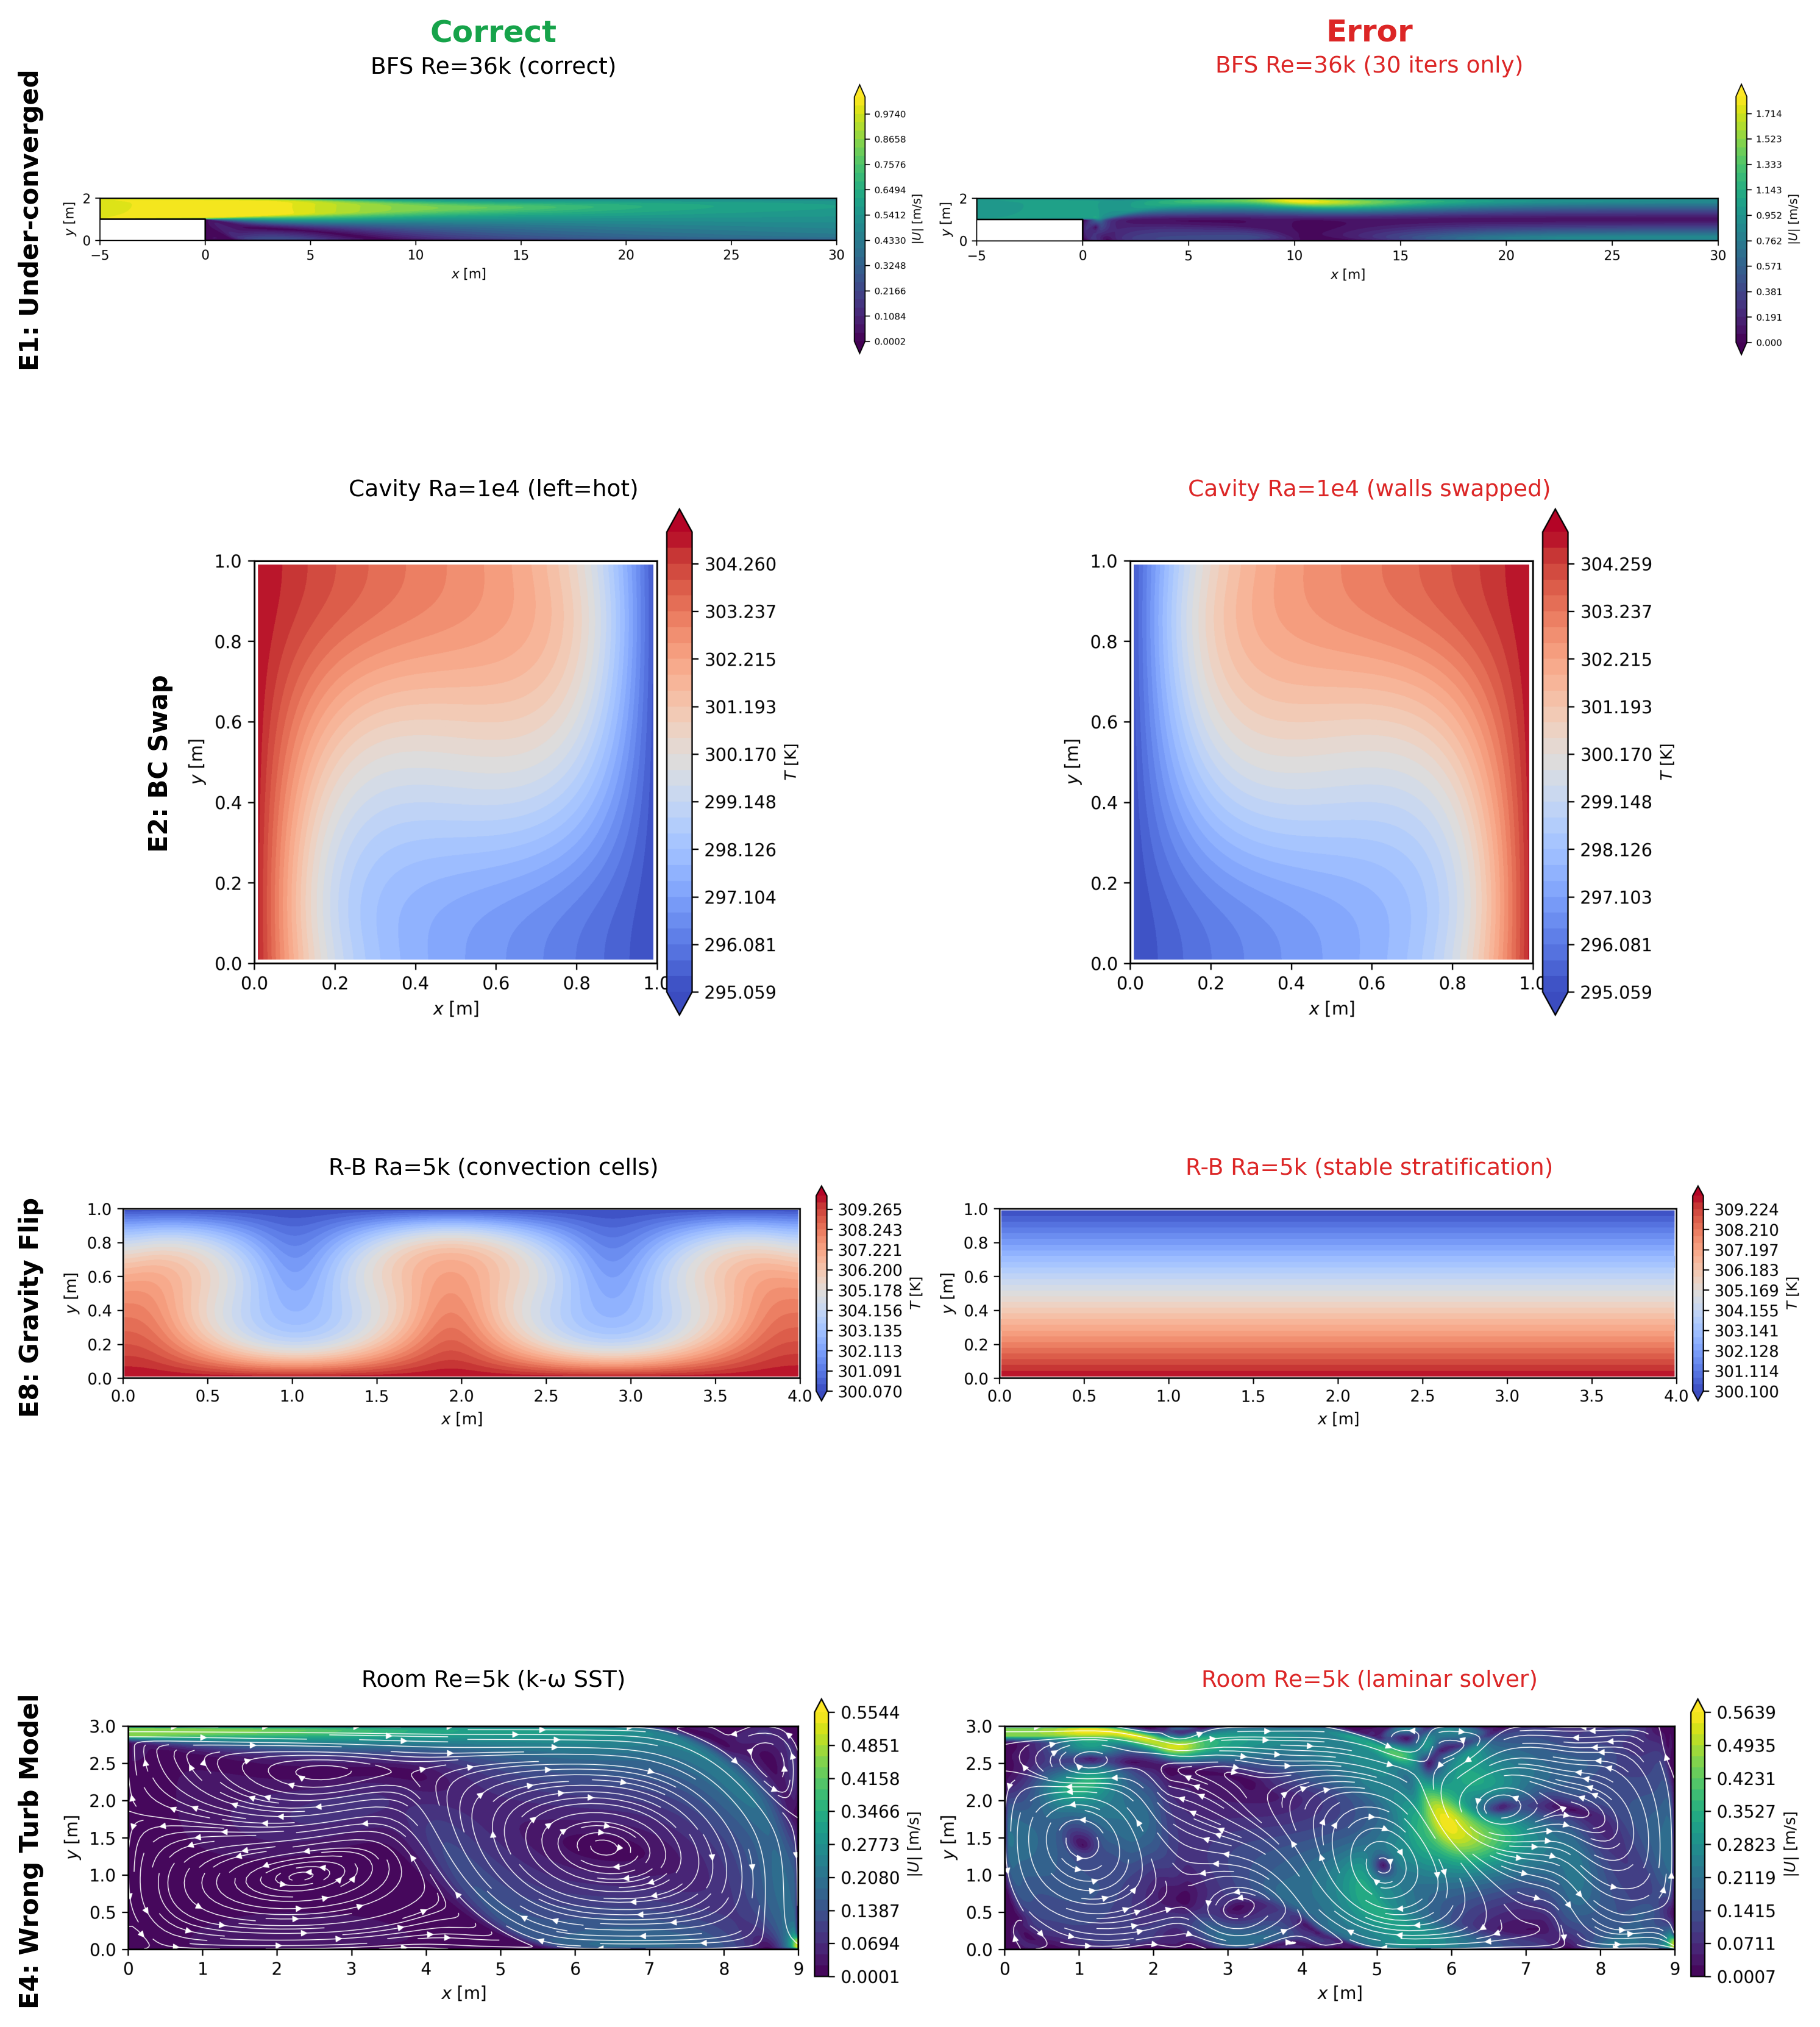
\includegraphics[width=\textwidth]{fig_error_examples.png}
\caption{Representative correct (left) vs.\ error (right) flow fields for four error types. Top to bottom: E1 under-convergence, E2 BC swap, E8 gravity flip, E4 wrong turbulence model.}
\label{fig:error-examples}
\end{figure}

\subsection{Evaluation Protocol}

We implement a blind, setup-conditioned protocol (Fig.~\ref{fig:eval-protocol}): evaluators receive problem setup text and anonymized flow field images, judging physical plausibility without access to ground truth labels.

\begin{figure}[htbp]
\centering
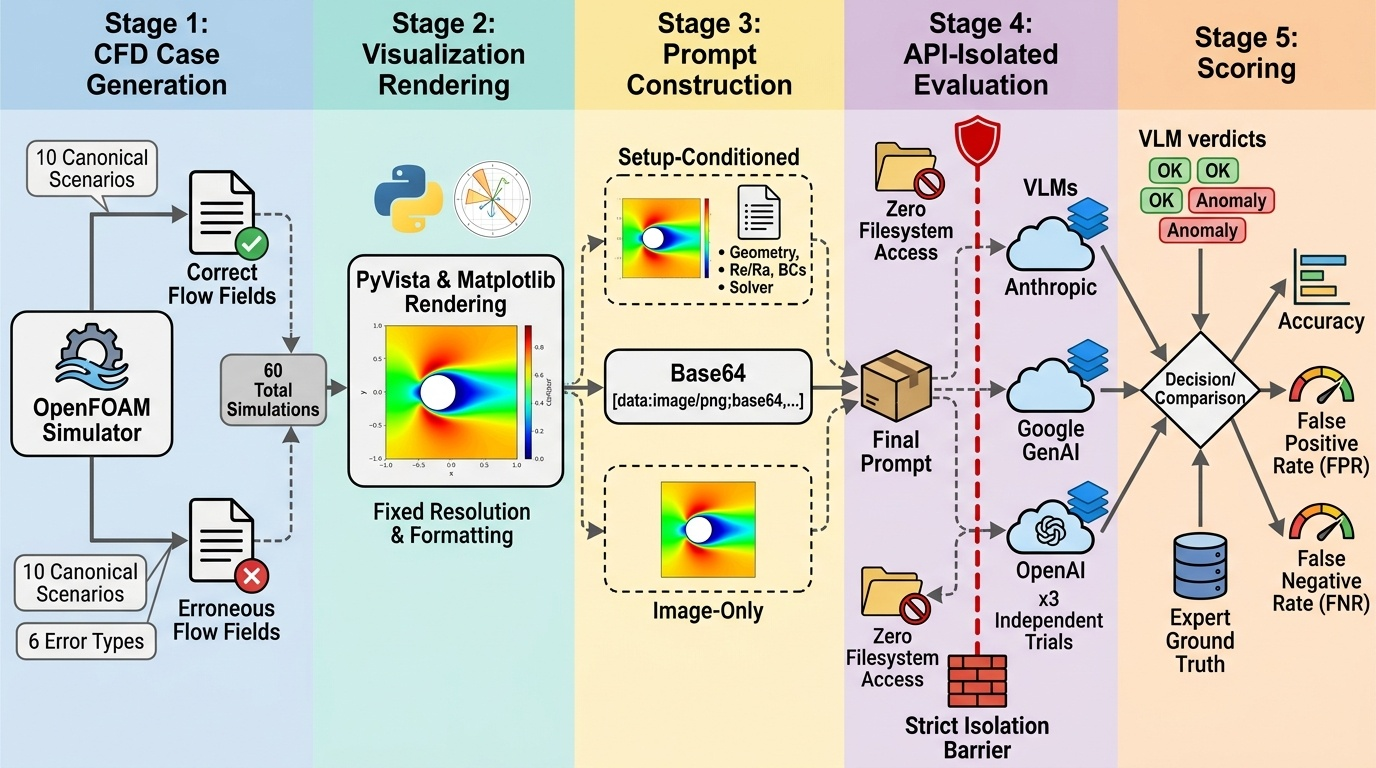
\includegraphics[width=\textwidth]{fig_eval_protocol.png}
\caption{Blind evaluation protocol: CFD case generation $\to$ visualization with anonymized codes $\to$ setup-conditioned prompt $\to$ independent blind evaluation $\to$ scoring.}
\label{fig:eval-protocol}
\end{figure}

\section{Results}

\subsection{Overall Performance}

Table~\ref{tab:main-results} and Fig.~\ref{fig:main-results} summarize the overall accuracy. Claude Opus 4.6 achieves 98.7\% on 75 items (single false positive on a complex wake pattern). The domain expert achieves 73.8\% on 80 items with 19 false negatives. Gemini 3.1 achieves 86.2\% on valid responses (25/29).

\begin{table}[htbp]
\centering
\caption{Overall evaluation performance.}
\label{tab:main-results}
\begin{tabular}{lrrrrr}
\toprule
Evaluator & Items & Accuracy & FP & FN & No-resp. \\
\midrule
Claude Opus 4.6 & 75 & 98.7\% & 1 & 0 & 0\% \\
Gemini 3.1 & 29 & 86.2\% & 2 & 2 & 3\% \\
Domain Expert & 80 & 73.8\% & 2 & 19 & 0\% \\
\bottomrule
\end{tabular}
\end{table}

\begin{figure}[htbp]
\centering
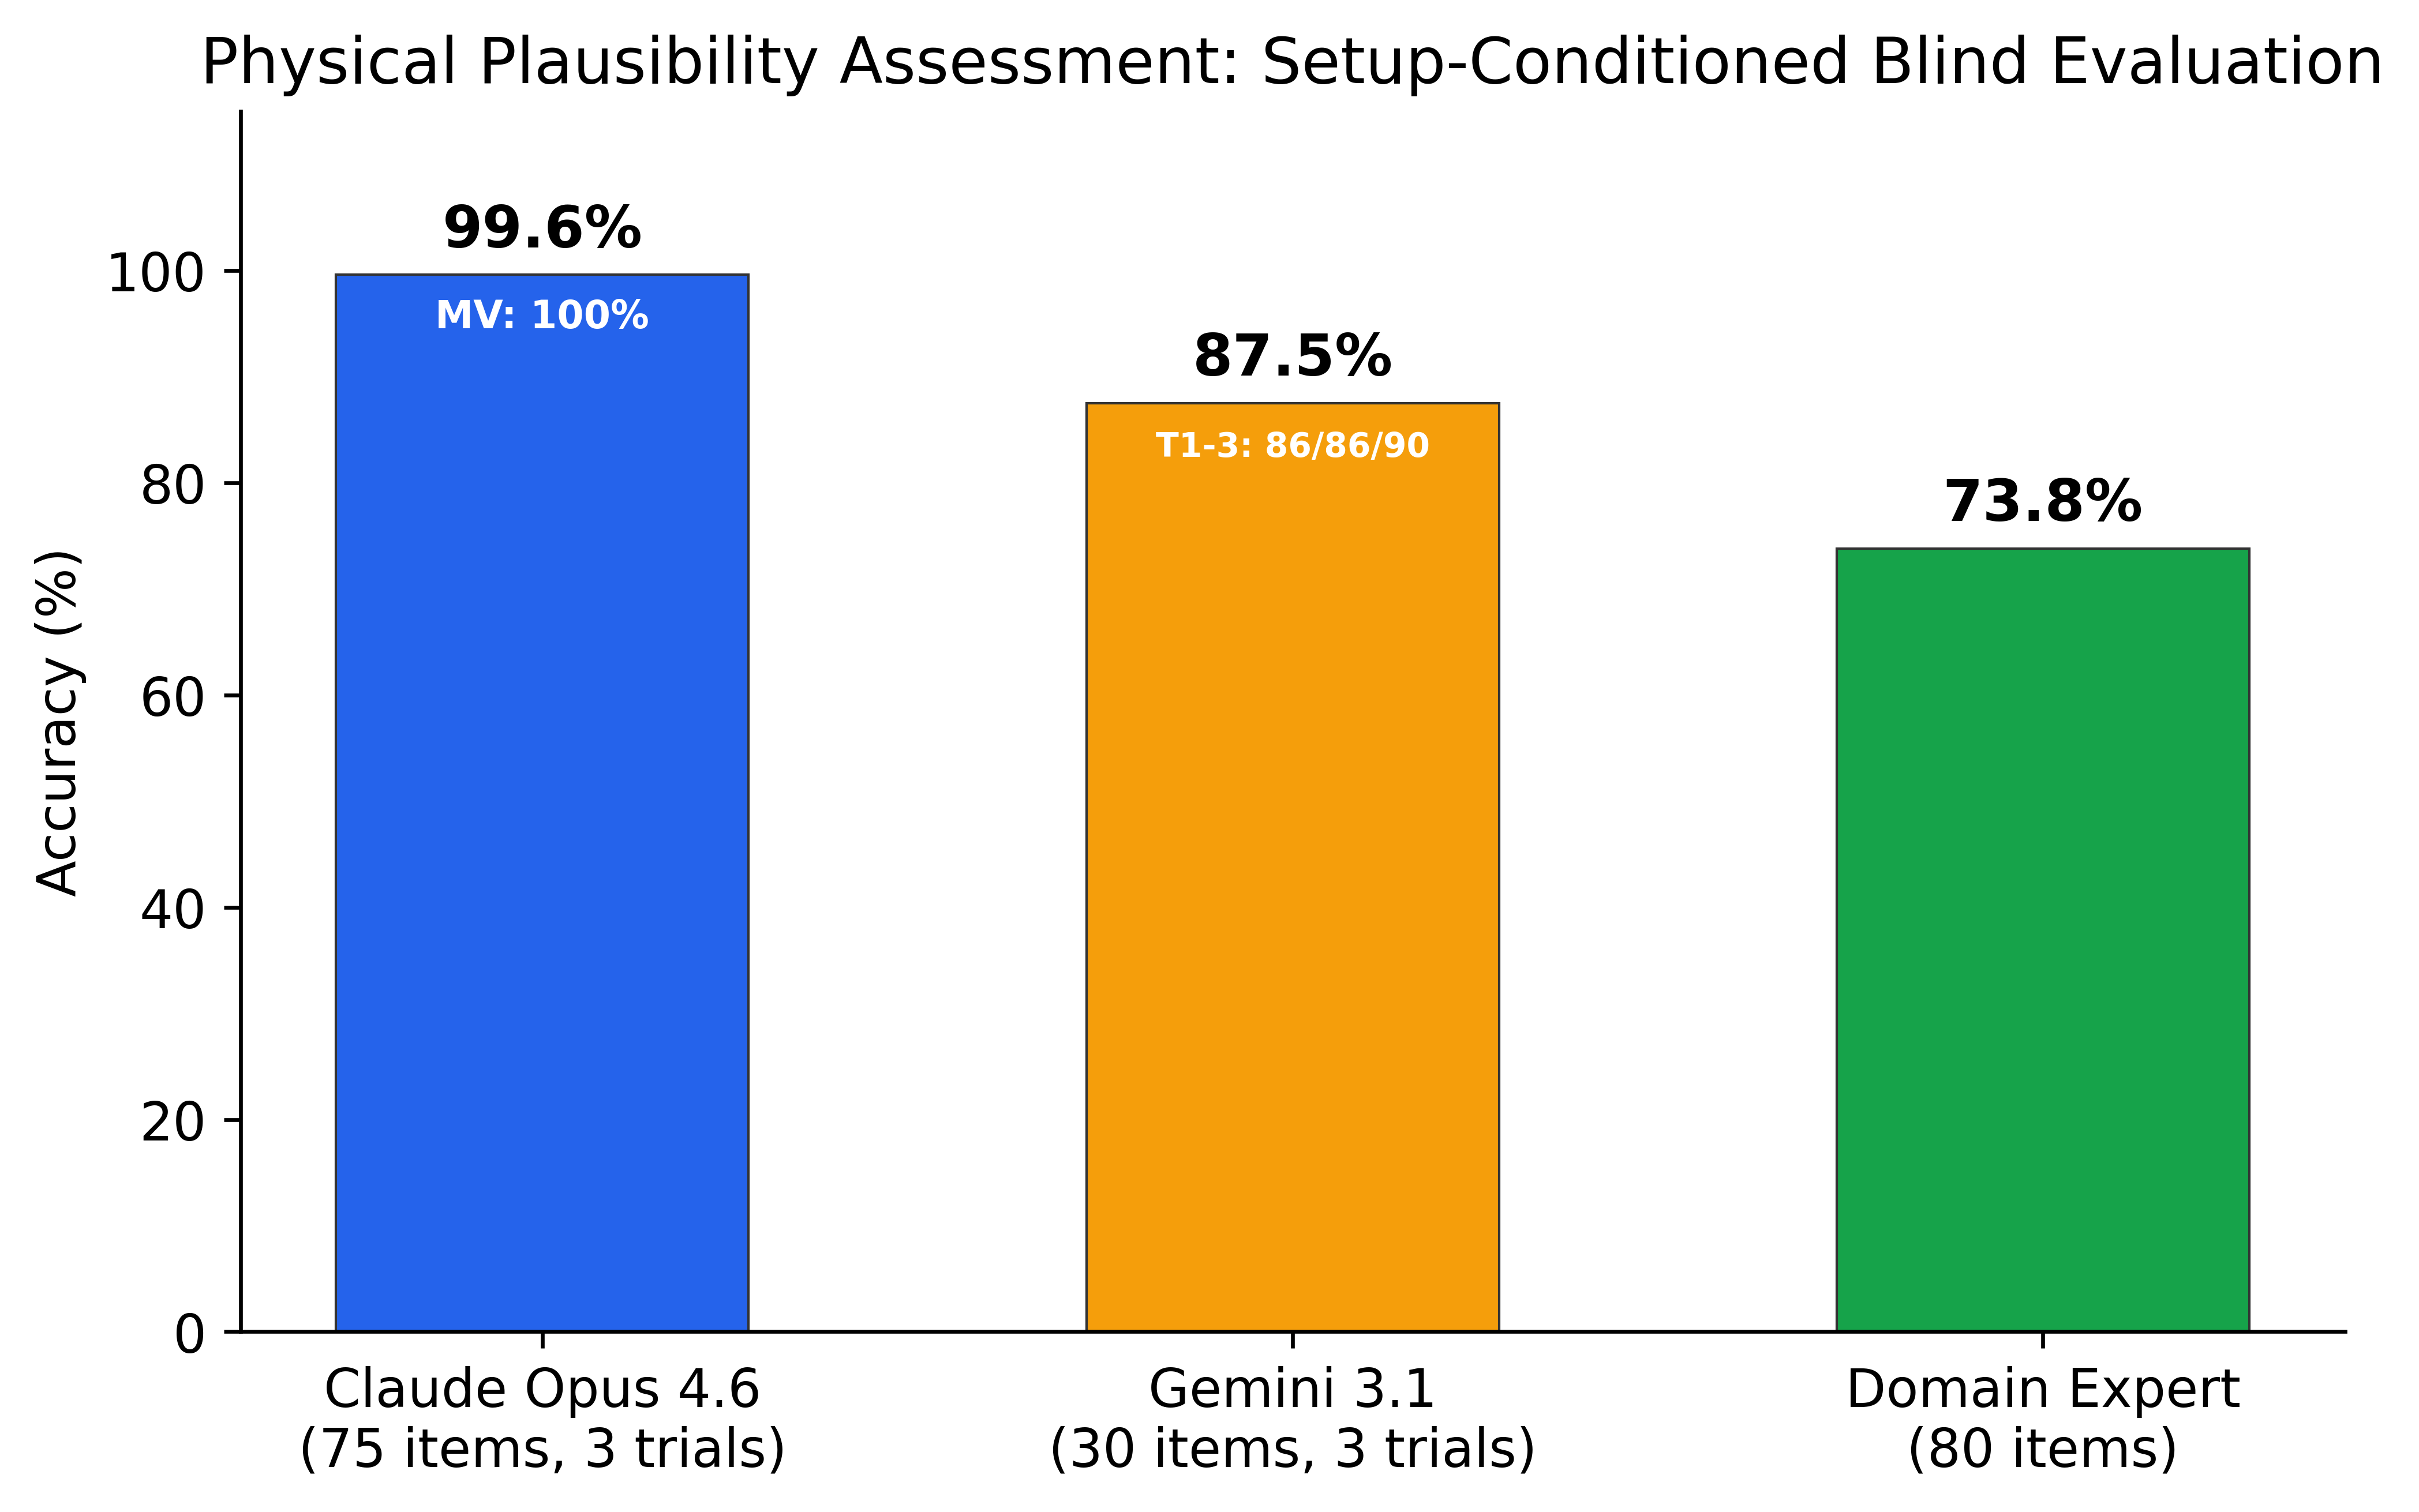
\includegraphics[width=0.8\textwidth]{fig_main_results.png}
\caption{Physical plausibility assessment accuracy by evaluator. Claude Opus 4.6 mean accuracy across 3 trials: 99.6\%; Gemini 3.1 mean: 87.5\%; Domain Expert: 73.8\%.}
\label{fig:main-results}
\end{figure}

\subsection{Per-Error-Type Analysis}

Fig.~\ref{fig:error-heatmap} shows error detection rates by type. The expert's primary blind spots are E2 boundary condition swap (20\% recall) and E3 wrong viscosity (29\%), while Claude achieves 100\% recall across all error types.

\begin{figure}[htbp]
\centering
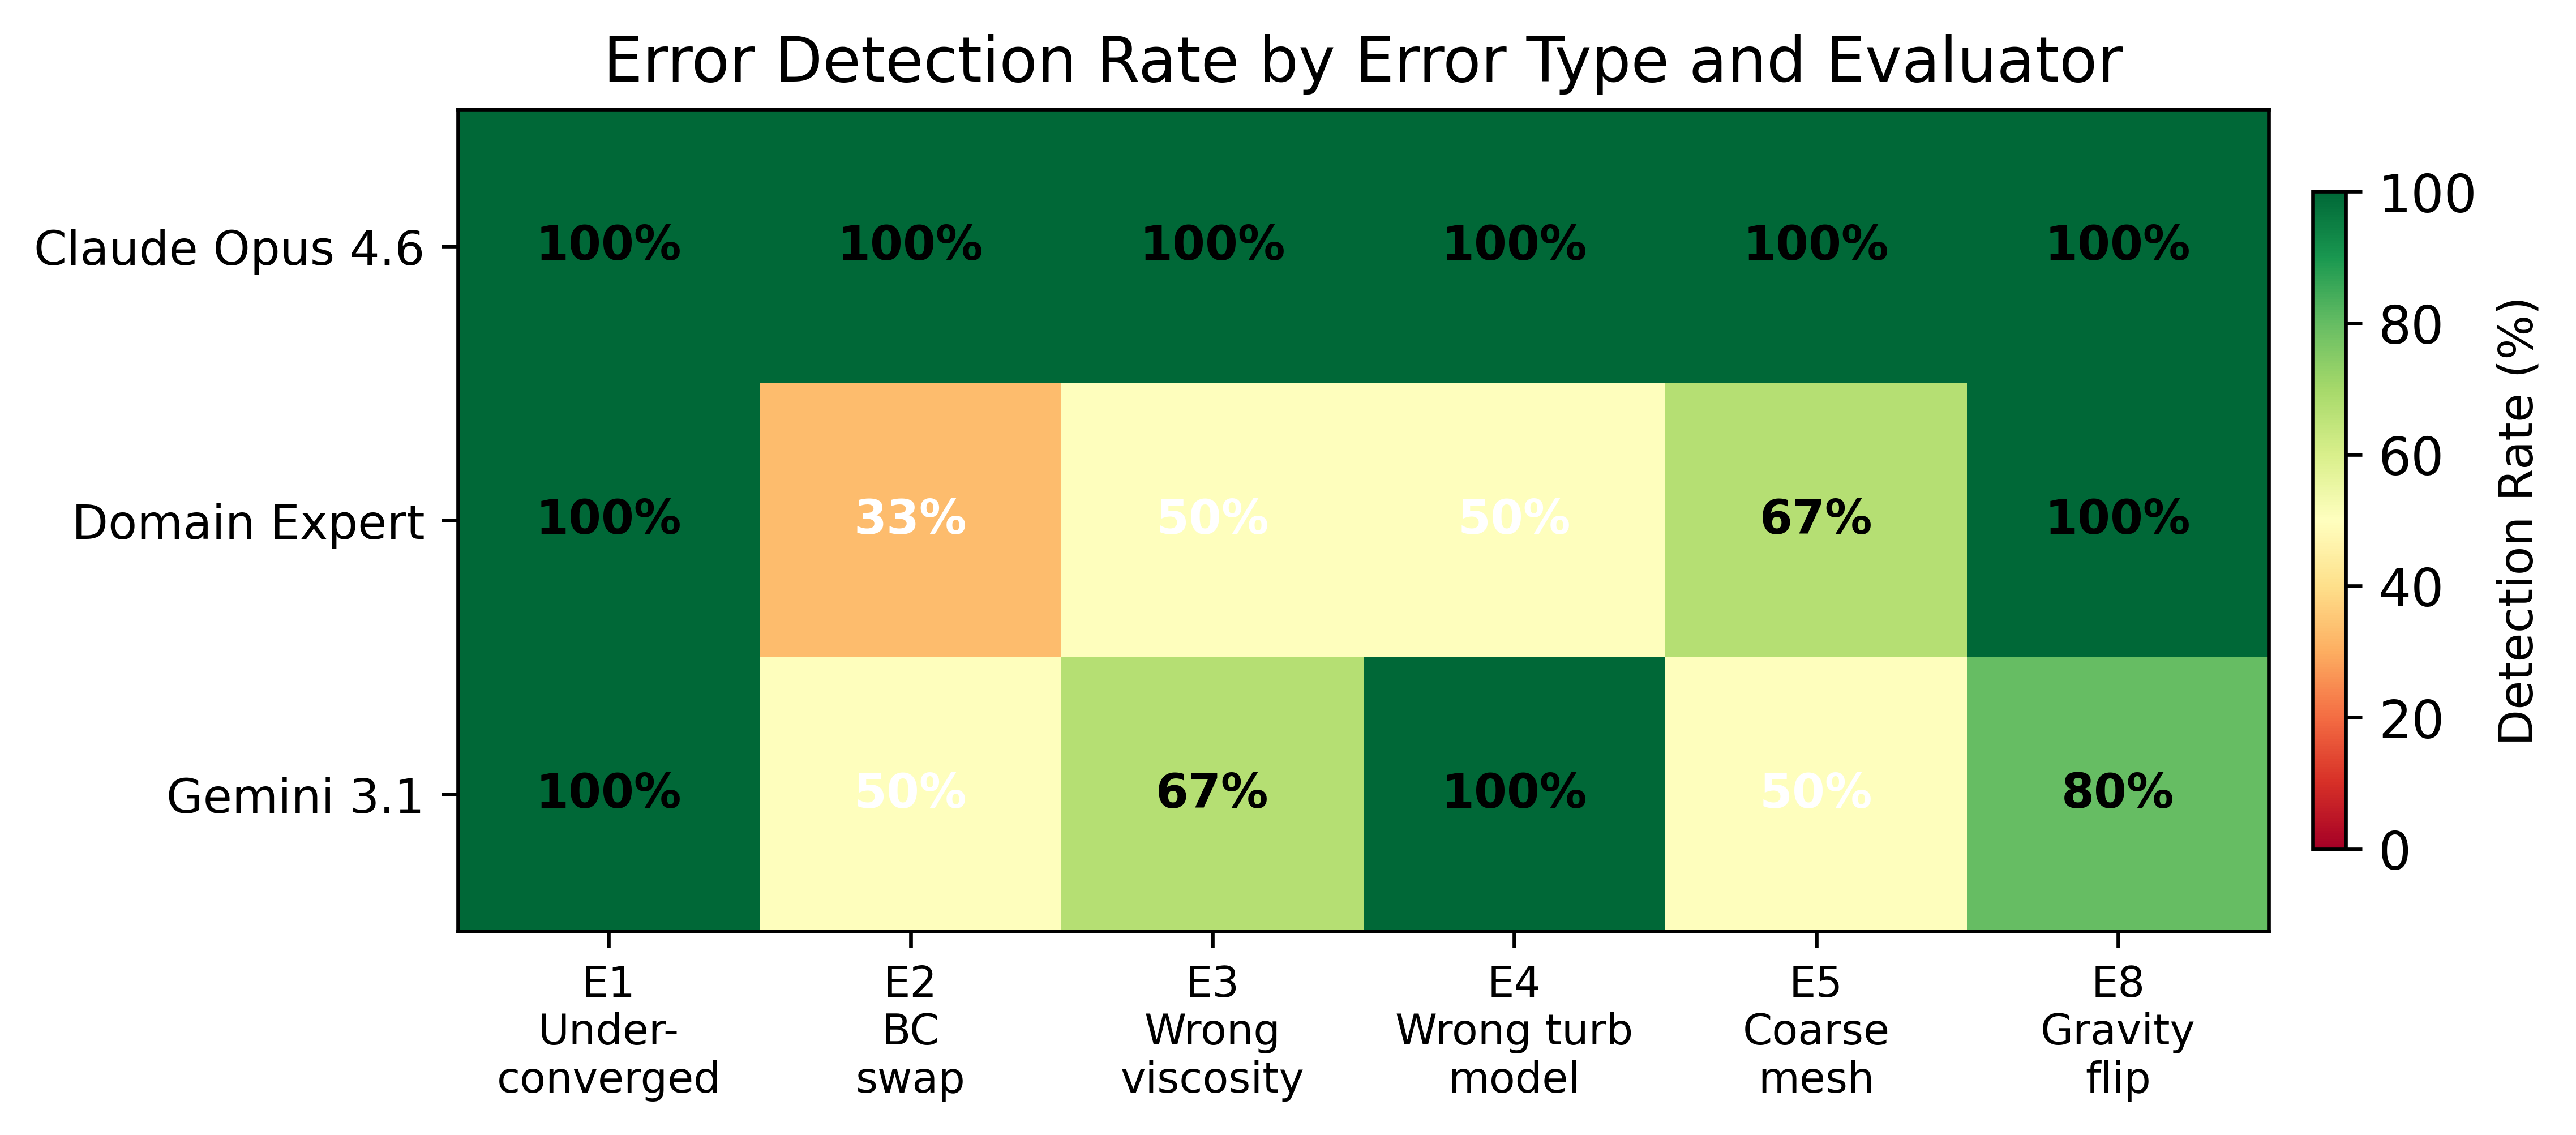
\includegraphics[width=\textwidth]{fig_error_heatmap.png}
\caption{Error detection rate by error type and evaluator. Claude detects all error types; the expert struggles with BC swap and wrong viscosity.}
\label{fig:error-heatmap}
\end{figure}

\subsection{Multi-Trial Consistency}

Three independent blind evaluations of Claude Opus yield 98.7\%, 100\%, and 100\% accuracy (Fig.~\ref{fig:trials-contamination}a). Across 225 judgments, 224 were correct (99.6\%). The single false positive was not reproduced, confirming it as stochastic. Majority vote achieves 100\%.

\subsection{Contamination Paradox}

An initial non-blind evaluation achieved 87\%, while blind evaluation achieved 100\% (Fig.~\ref{fig:trials-contamination}b). We hypothesize that case-name metadata triggers anchoring bias, while blind conditions force systematic cross-referencing.

\begin{figure}[htbp]
\centering
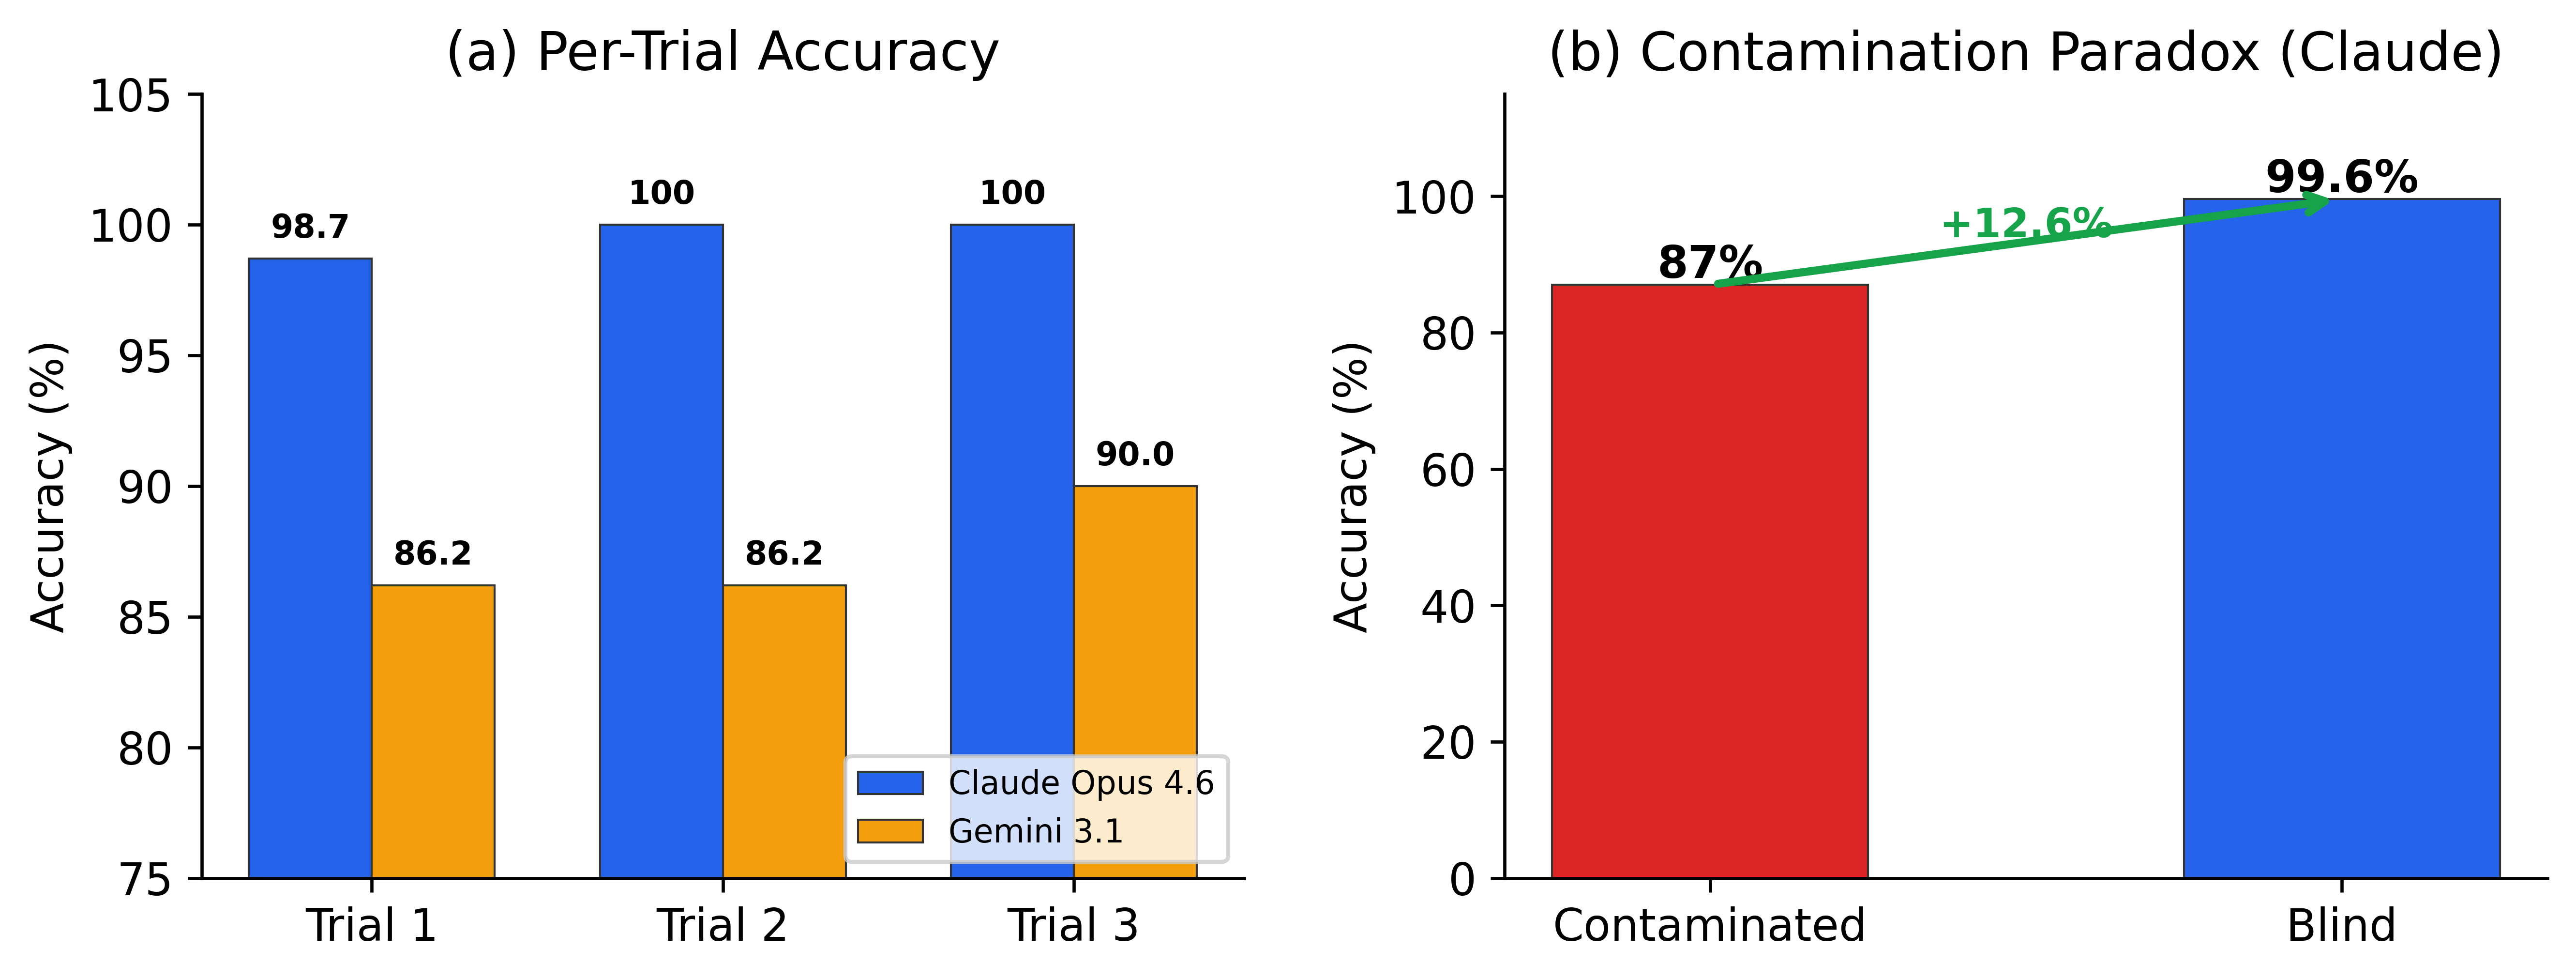
\includegraphics[width=\textwidth]{fig_trials_contamination.png}
\caption{(a) Per-trial accuracy for Claude and Gemini across 3 independent trials. (b) Contamination paradox: blind evaluation outperforms non-blind for Claude Opus.}
\label{fig:trials-contamination}
\end{figure}

\subsection{Setup-Conditioned vs.\ Image-Only Evaluation}

To quantify the importance of problem setup information, we evaluated Claude Opus and Gemini 3.1 on 30 items under two conditions: setup-conditioned (with problem description) and image-only (no setup text). Claude drops from 98.7\% to 83.3\% ($-$15.4\,pp) and Gemini from 87.5\% to 79.2\% ($-$8.3\,pp). In image-only mode, Claude misses 5 errors it detects with setup: wrong viscosity (2 cases), wrong turbulence model, reversed lid direction, and coarse mesh --- precisely the error types where the image alone appears physically self-consistent. For example, a boundary condition swap (S6\_E2) produces a valid-looking differentially heated cavity with swapped orientation; only comparison with the stated wall temperatures reveals the error. This confirms that CFD validation is fundamentally setup-conditioned, and VLM-based validators must receive simulation parameters alongside the image.

\section{Discussion}

The most striking result is that Claude Opus detects error types that the domain expert consistently misses. We attribute this to a difference in evaluation strategy: the expert employs gestalt assessment (``does this look right?''), while the VLM systematically cross-references stated boundary conditions against observable image features. This suggests complementary capabilities: an ensemble approach combining VLM parameter checking with expert holistic judgment could achieve higher coverage than either alone.

Limitations include sample size (75--80 items per evaluator), single expert baseline, two VLMs tested, and restriction to 2D steady-state flows. The benchmark should be extended to 3D visualizations, transient flows, and additional VLM architectures.

\section{Conclusion}

We introduced CFD-VisQA, the first benchmark for evaluating VLM capabilities in CFD flow field plausibility assessment. Claude Opus 4.6 achieves 99.6\% accuracy across 225 judgments with 100\% majority vote, detecting all error types including those the domain expert misses (BC swap: 20\% expert recall, wrong viscosity: 29\%). The contamination paradox and multi-trial consistency findings provide practical guidance for deploying VLMs as automated CFD validators. The benchmark dataset and evaluation pipeline are publicly available.

\section*{Data Availability}

The CFD-VisQA benchmark dataset, evaluation scripts, and VLM response transcripts are available at \url{https://github.com/yhjoo-kier/OpenFOAM} (branch: \texttt{paper/cfd-visual-qa}).

\section*{Declaration of Competing Interests}

The authors declare no competing interests.

%% Temporary bibliography - replace with .bib when Zotero keys are ready
\begin{thebibliography}{99}
\bibitem{joo2026} Joo et al., Image-to-CFD framework, 2026.
\bibitem{yue2024mmmu} Yue et al., MMMU: A massive multi-discipline multimodal understanding benchmark, CVPR 2024.
\bibitem{pandey2025} Pandey and Ottley, Benchmarking VLMs on visualization literacy tests, EuroVis 2025.
\bibitem{chow2025physbench} Chow et al., PhysBench: Physical world understanding benchmark, ICLR 2025.
\bibitem{chen2024climateIQA} Chen et al., ClimateIQA: Meteorological heatmap VLM benchmark, 2024.
\bibitem{kashefi2024} Kashefi, A misleading gallery of fluid motion by generative AI, arXiv:2405.15406, 2024.
\bibitem{somasekharan2025} Somasekharan et al., CFDLLMBench, arXiv:2509.20374, 2025.
\bibitem{mdpi2026vlmcfd} VLM for indoor CFD mixed reality, MDPI Technologies, 2026.
\bibitem{roberts2024} Roberts et al., SciFIBench, NeurIPS 2024.
\end{thebibliography}

\end{document}
